\documentclass[a4paper,12pt]{report}
\usepackage[left=1cm,right=1cm,top=3cm,bottom=3cm,a4paper]{geometry}
\usepackage[pdftex]{graphicx}
\usepackage{graphicx}\usepackage{amsmath}
\usepackage{amsfonts}
\usepackage{amssymb}
\usepackage{kotex}
\newcommand{\Maxwell}[3][]{\left.\frac{\partial #2}{\partial #3} \right)_{#1} }
\newcommand{\dbar}{d\hspace*{-0.08em}\bar{}\hspace*{0.1em}}
\usepackage[onehalfspacing]{setspace}
\begin{document}
	\chapter*{4장 열역학 함수}
	\paragraph{4-1.} 스핀이 s=1/2인 자성원자 $N$개로 이루어진 계가 있다. 충분한 고온에서는 자성원자들이 완전히 마구잡이로 정렬하지만, $T\rightarrow0$ 인 극저온에서는 모든 자성원자들이 한 방향으로만 정렬한다. 어떤 근사 이론에서 고체의 비열이 온도에 따라 다음과 같이 변한다. 
	$$ C(T)=\begin{cases} C_1\left(\frac{2T}{T_1}-1 \right)&T_1/2<T<T_1\\0 & \mbox{otherwise.}\end{cases}$$
	한편, 고체의 조성비를 조절하여 $N$개의 자성원자 중 $30 \% $ 를 비자성 원자로 바꾸면 비열의 온도 의존성이 다음과 같이 변한다. 
	$$C(T)=\begin{cases}C_2\left( \frac{2T}{T_2}\right)&0<T<T_2 \\0&\mbox{otherwise. }	\end{cases}$$
	(ㄱ) 엔트로피의 변화를 이용하여 비례상수 $C_1$을 구하여라.\\
	(ㄴ) $T_2<T_1$ 인 이유를 설명하여라.\\
	(ㄷ) $C_2/C_1$의 비를 구하여라.
	\subparagraph{풀이}(ㄱ) 주어진 고체는 충분한 고온 ($T_1$) 에서는 자성원자들이 $\uparrow $ 또는 $\downarrow$ 방항으로 완전하게 랜덤하게 정렬하고, 저온 ($T_1/2$)에서는 한 방향으로만 정렬한다. 따라서 온도 $T_1$ 에서 엔트로피는 $k_B\ln(2^N)=Nk_B\ln2$이고, $T_1/2$ 에서 엔트로피는 $k_B\ln(1^N)=0$ 이다. 그러면 비열의 정의에 의해,
	$$C=T\frac{dS}{dT},\quad dS=\frac{C}{T}dT$$
	 \begin{equation}
	\begin{split}
	\Delta S=\int_{T_1/2}^{T_1} \frac{C}{T}dT & = \int_{T_1/2}^{T_1} C_1\left( \frac{2T}{T_1}-1\right) \frac{1}{T}dT \\
	& = \int_{T_1/2}^{T_1} C_1\left( \frac{2}{T_1}-\frac{1}{T}\right)dT\\
	&= C_1\left[\frac{2}{T_1}T-\ln T \right]_{T_1/2}^{T_1} \\
	&= C_1(1-\ln 2)=Nk_B\ln 2
	\end{split}
	\end{equation}
	따라서, 
	$$  C_1=\frac{Nk_B\ln 2}{1-\ln 2}$$
	(ㄴ)  자성원자들의 상호작용으로 비열이 0이 아닌 값을 갖게 되는데, $30\%$를 비자성원자로 바꾸면 자성원자들의 상호작용이 줄어들므로 유한한 비열값이 생기는 온도가 낮아지고, $T\rightarrow0$ 에서 $C\rightarrow0$ 이 되는 변화가 보다 서서히 일어나게 될 것이다. \\
	(ㄷ) 자성원자 조성비를 $0.7N$으로  바꾼 후에는 충분한 고온 ($T_2$)에서 완전하게 랜덤하게 정렬하고 극저온 $(T=0)$에서 한 방향으로만 정렬하므로, 온도 $T_2$에서 엔트로피는 $k_B\ln (2^{0.7N})=0.7Nk_B\ln2$ 이고 온도 $T=0$에서 엔트로피는 $k_B\ln(1^{0.7N})=0$ 이다. (ㄱ)에서와 마찬가지로, 
	\begin{equation}
	\begin{split}
	\Delta S=\int_{0}^{T_2} \frac{C}{T}dT &=\int_{0}^{T_2}C_2\left(\frac{2T}{T_2} \right)\frac{1}{T}dT \\
	& = \int_{0}^{T_2}C_2\left(\frac{2}{T_2} \right)dT\\
	& = 2C_2=0.7Nk_B\ln 2
	\end{split}
	\end{equation}
	따라서, 
	$$C_2/C_1=\frac{(0.7Nk_B\ln 2) / 2}{(Nk_B\ln 2)/(1-\ln 2)}=0.35(1-\ln2)$$
	\paragraph{4-2. } 이상기체의 엔탈피가 
	$$H(S,P,N)=\frac{5}{3}U_0\left(\frac{N}{N_0} \right)\left(\frac{P}{P_0} \right)^{2/5}\exp\left[\frac{2}{5}\left(\frac{S}{Nk_B}-S_0 \right) \right]  $$
	임을 보이고, 상태방정식과 내부에너지를 구해라.
	\subparagraph{풀이} 열역학 제 1법칙에서 
	$$dU=TdS-PdV,\quad dS=\frac{1}{T}dU+\frac{P}{T}dV=\frac{3}{2}Nk_B\frac{dT}{T}+Nk_B\frac{dV}{V} $$에서,
	$$\Delta S=\frac{3}{2}Nk_B\ln(T/T_0)+Nk_B\ln(V/V_0)$$
	$$S(T,V)-S_0(T_0,V_0)=Nk_B\ln\left[\left(\frac{T}{T_0}\right)^{3/2}\left(\frac{V}{V_0}\right)\right]$$
	이것을 $T,P$에 대한 함수로 바꾸면,($PV/T=$일정)
	$$S(T,P)-S_0(T_0,P_0)=Nk_B\ln\left[\left(\frac{T}{T_0}\right)^{3/2}\left(\frac{TP_0}{PT_0}\right)\right]$$
	$$S(T,P)-S_0(T_0,P_0)=Nk_B\ln\left[\left(\frac{T}{T_0}\right)^{5/2}\left(\frac{P_0}{P}\right)\right]$$
	$S_0=Nk_Bs_0$이라고 하면,
	$$S(N,T,P)=Nk_B\left(s_0+\ln\left[\left(\frac{T}{T_0} \right)^{5/2} \left(\frac{P_0}{P} \right) \right] \right) $$
	이상기체의 경우 $U=(3/2)Nk_BT$ 이므로,
	$$\frac{T}{T_0}=\frac{N_0U}{U_0N}$$
	에서, 
	$$S(N,U,P)=Nk_B\left(s_0+\ln\left[\left(\frac{N_0U}{NU_0} \right)^{5/2} \left(\frac{P_0}{P} \right) \right] \right) $$
	이제 이것을 내부에너지에 대한 식으로 바꾸자.
	$$\rightarrow \, \left( \frac{S}{Nk_B}-s_0\right)=\ln\left[\left(\frac{U}{U_0} \right)^{5/2} \left(\frac{N_0}{N} \right)^{5/2} \left(\frac{P_0}{P} \right)  \right]  $$
	$$\rightarrow \, \left(\frac{P}{P_0} \right)^{2/5} \left(\frac{N}{N_0} \right) \exp\left[\frac{2}{5}\left( \frac{S}{Nk_B}-s_0\right)\right]=\frac{U}{U_0}  $$
	$$U(S,P,N)=U_0\left(\frac{P}{P_0} \right)^{2/5} \left(\frac{N}{N_0} \right) \exp\left[\frac{2}{5}\left( \frac{S}{Nk_B}-s_0\right)\right]$$
	한편, $H=U+PV$ 에서 이상기체의 경우 $PV=(2/3)U$ 이므로, $H=(5/3)U$ 이다. 따라서,
	$$H(S,P,N)=\frac{5}{3}U(S,P,N)=\frac{5}{3}U_0\left(\frac{P}{P_0} \right)^{2/5} \left(\frac{N}{N_0} \right) \exp\left[\frac{2}{5}\left( \frac{S}{Nk_B}-s_0\right)\right]$$
	$dH=TdS+VdP$ 에서 
	$$T=\left. \frac{\partial H}{\partial S}\right) _{P,N},\quad V=\left.\frac{\partial H}{\partial P} \right)_{S,N} $$ 이므로,
	$$T=\left. \frac{\partial H}{\partial S}\right) _{P,N}=\frac{2}{5Nk_B}H$$
	$$V=\left.\frac{\partial H}{\partial P} \right)_{S,N} =\frac{2}{5P}H$$
	두 식을 정리하면,
	$$H=\frac{5k_BT}{2}=\frac{5PV}{2}=\frac{5U}{3},\quad PV=Nk_BT,\quad U=\frac{3}{2}Nk_BT$$
	\paragraph{4-3. }$$H=G-T\left. \frac{\partial G}{\partial T}\right) _P=-T^2\left. \frac{\partial G/T}{\partial T}\right) _P$$ 임을 보여라. 이 식을 Gibbs-Helmholtz 방정식이라고 부른다. 
	\subparagraph{풀이}$$\begin{cases}
	H=U+PV,&dH=TdS+VdP\\G=U-TS+PV,&dG=-SdT+VdP
	\end{cases}$$
	$$H=G+TS=G-T\left(\frac{\partial G}{\partial T} \right)_P=-T^2\left(\frac{\partial}{\partial T}\left( \frac{G}{T}\right)\right)_P  $$
	note that 
	$$\left(\frac{\partial}{\partial T}\left( \frac{G}{T}\right)\right)_P=\frac{1}{T}\frac{\partial G}{\partial T}-\frac{G}{T^2}$$
	\paragraph{4-4. } 어떤 열역학 계의 상태방정식이 $P^2e^{aV}=bT^{1/3}$ 으로 주어진다. 단 $a,b$ 는 상수이다. \\
	(ㄱ) 등온압축률 $\chi(T,V,P)$를 구하여라.\\
	(ㄴ) 등압팽창률 $\beta(T,V,P)$를 구하여라.
	\subparagraph{풀이} 양변을 미분하면 
	$$2Pe^{aV}dP+aP^2e^{aV}dV=\frac{b}{3}T^{-2/3}dT=\frac{b}{3}\frac{T^{1/3}}{T}dT$$ 
	$$2Pe^{aV}dP+aP^2e^{aV}dV=\frac{b}{3}\frac{P^{2}e^{aV}/b}{T}dT=\frac{P^{2}e^{aV}}{3T}dT$$ 
	정리하면,
	$$2\frac{dP}{P}+adV=\frac{1}{3}\frac{dT}{T}$$
	$$dV=\left(\frac{1}{3a} \right)\frac{dT}{T}-\left( \frac{2}{a}\right) \frac{dP}{P} $$
	(ㄱ) 등온압축률
	$$\chi=-\frac{1}{V}\left. \frac{\partial V}{\partial P}\right)_T=-\frac{1}{V}\left( -\frac{2}{aP}\right) =\frac{2}{aPV} $$
	(ㄴ) 등압팽창률
	$$\beta=\frac{1}{V}\left. \frac{\partial V}{\partial T}\right)_P=\frac{1}{V}\left(\frac{1}{3aT} \right)=\frac{1}{3aVT}  $$
	\paragraph{4-5. } 열역학 제 1법칙을 이용하여 $V(U,S), V(P,S), V(P,T)$ 표현식을 구하되, 가능하면 Maxwell relation을 이용해 $C_V, C_P, \chi, \beta$를 포함시켜라. 단 $dN=0$이다.
	\subparagraph{풀이} (ㄱ) 열역학 제 1법칙 $dU=TdS-PdV$ 에 의해
	$$dV(U,S)=\frac{T}{P}dS-\frac{1}{P}dU$$
	(ㄴ) $V(P,S)$ 의 변수가 $P,S$로 주어졌으므로 $dP,dS$를 통해  $dV$를 전개하자.
	$$dV(P,S)=\left. \frac{\partial V}{\partial P}\right) _{S}dP+\left.\frac{\partial V}{\partial S} \right)_{P}dS $$ 엔트로피에 대한 미분은 Maxwell relation을 통해 우리가 실험적으로 쉽게 다룰 수 있는 미분으로 바꿀 수 있다. 
	$$\left. \frac{\partial V}{\partial S}\right)_P \mbox{ 에 연관된 열역학 변수는 }S,P $$
	이므로, $dN=0$ 일 때 $dS,dP$를 변수로 갖는 열역학 함수가 무엇이 있는지 생각해보면 엔탈피가 있다. ($dH=TdS+VdP$) Maxwell relation은 $\partial_S, \, \partial_P$ 은 그대로 두고 $T,V$의 자리를 바꿔주면 나온다. 
	$$\partial_S V|_P=\partial_P T|_S \quad\rightarrow\left. \frac{\partial V}{\partial S}\right)_P=\left. \frac{\partial T}{\partial P}\right)_S=\left. \frac{\partial T}{\partial V}\right)_S\left. \frac{\partial V}{\partial P}\right)_S $$ 
	위의 결과를 전개식에 대입하면
	$$dV(P,S)=\left. \frac{\partial V}{\partial P}\right) _{S}dP+\left. \frac{\partial T}{\partial V}\right)_S\left. \frac{\partial V}{\partial P}\right)_SdS $$
	$$dV(P,S)=\left. \frac{\partial V}{\partial P}\right) _{S}\left[ dP+\left. \frac{\partial T}{\partial V}\right)_S dS\right] $$
	인데, 
	\begin{equation*}
	\begin{split}0=dS(T,V)&=\Maxwell[V]{S}{T}dT+\Maxwell[T]{S}{V}dV\\
	&=\frac{C_V}{T}dT+\Maxwell[V]{P}{T}dV \end{split}
	\end{equation*}
	여기서  $\partial P/\partial T|_V$은 $\partial S/\partial V|_T$  을 Maxwell relation을 이용해서 바꾼 것이다. 따라서,
	$$-\frac{C_V}{T}dT=\Maxwell[V]{P}{T}dV, \quad dS=0$$
	에서 양변을 $dV$로 나누면,
	$$\Maxwell[S]{T}{V}=-\frac{T}{C_V}\Maxwell[V]{P}{T}$$
	이므로 다음과 같이 나타낼 수 있다.
	$$dV(P,S)=\Maxwell[S]{V}{P}\left[ dP-\frac{T}{C_V}\Maxwell[V]{P}{T}dS\right] $$
	(ㄷ)
	$$dV(P,T)=\Maxwell[T]{V}{P}dP+\Maxwell[P]{V}{T}dT=V(-\chi dP+\beta dT)$$
	(ㄴ),(ㄷ) 문제는 기본적으로 변수변환의 문제이다. 즉, $(U,S)\rightarrow(P,S)$ 및 $(U,S)\rightarrow(P,T)$ 변환문제이다. 이러한 변수변환은 Jacobi 행렬식을 이용한 Jacobi 변환식을 이용하면 된다. 그후 Maxwell relation을 통해 $C_V,C_P,\chi, \beta$ 를 포함시킬 수 있다. 그러나 그 표현은 어떤 실험조건이냐에 따라 최종 표현식을 이끌어내야 하므로 위의 결과는 여러 표현 중의 하나일 뿐이다. 
	\paragraph{4-6. } 기체가 임의의 열역학 과정에서 한 일을
	 $$\dbar W=PV\beta dT-PV\chi dP$$
	 로 쓸 수 있음을 보이고, 이 식을 이용하여 이상기체가 임의의 열역학 과정에서 한 일의 표현을 구하여라.
	 \subparagraph{풀이} 기체에서 일은 일반적으로 
	 $$\dbar W=PdV$$ 로 쓸 수 있다. 그런데 $V$를 $T,P$ 의 함수 $V(T,P)$ 로 보면
	 $$\dbar W=PdV(T,P)=P\left[\Maxwell[P]{V}{T}dT+\Maxwell[T]{V}{P}dP \right] $$
	 가 되는데 $\beta, \chi$ 의 정의로부터,
	 $$\dbar W=P(V\beta dT-V\chi dP)=PV\beta dT-PV\chi dP$$
	 이상기체의 경우 $\beta=1/T,\,\chi=1/P$ 를 만족하므로,
	 $$\dbar W_{ideal \,gas}=\frac{PV}{T} dT-VdP=Nk_BdT-\frac{Nk_BT}{P}dP$$
	 \paragraph{4-7. }실제 기체는 두 분자 사이의 상호작용 때문에, 상태방정식이 판데르 발스 기체에 가깝다.(12장 참조) 한편, 판데르 발스 기체의 몰당 상태방정식은 다음과 같다. 
	 $$\left(p+\frac{a}{v^2} \right) \left(v-b \right)=RT $$
	 (ㄱ) 이 기체의 몰당 등온압축률과 등압팽창률이 각각
	 $$\beta=\frac{Rv^2(v-b)}{RTv^3-2a(v-b)^2},\quad \chi=\frac{v^2(v-b)^2}{RTv^3-2a(v-b)^2}$$임을 보여라.\\
	(ㄴ) 위 결과를 이용하여 비열이 
	$$c_p=c_v+\frac{R^2Tv^3}{RTv^3-2a(v-b)^2}$$ 임을 보여라.
	\subparagraph{풀이} (ㄱ) 
	$$\beta=\frac{1}{v}\Maxwell[P]{v}{T}=-\frac{1}{v}\frac{\partial p/\partial T|_v}{\partial p/\partial v|_T}$$
	$$\mbox{note that,  } 0=dp(v,T)=\Maxwell[T]{p}{v}dv+\Maxwell[v]{p}{T}dT$$
	이고 Van der waals 방정식을 압력에 대해 나타내면
	$$p=\frac{RT}{v-b}-\frac{a}{v^2}$$
	이므로, 
	$$\Maxwell[T]{p}{v}=-\frac{RT}{(v-b)^2}+\frac{2a}{v^3}$$
	$$\Maxwell[v]{p}{T}=\frac{R}{v-b}$$ 에서 
	$$\beta=\frac{1}{v}\Maxwell[P]{v}{T}=-\frac{1}{v}\frac{\partial p/\partial T|_v}{\partial p/\partial v|_T}=-\frac{1}{v}\frac{\frac{R}{v-b}}{-\frac{RT}{(v-b)^2}+\frac{2a}{v^3}}$$
	정리하면, 
	$$\beta=\frac{Rv^2(v-b)}{RTv^3-2a(v-b)^2}$$
	가 된다. 또,
	 $$\Maxwell[T]{p}{v}=-\frac{RT}{(v-b)^2}+\frac{2a}{v^3}=\frac{-RTv^3+2a(v-b)^2}{v^3(v-b)^2}$$ 으로부터
	 $$\chi=-\frac{1}{v}\Maxwell[T]{v}{p}=\frac{v^2(v-b)^2}{RTv^3-2a(v-b)^2}$$
	 (ㄴ)
	 $$c_p=c_v+Tv\frac{\beta^2}{\chi}$$ 에 (ㄱ)에서 구한 $\beta$ 와 $\chi$ 의 표현을 대입하면
	 $$c_p=c_v+\frac{R^2Tv^3}{RTv^3-2a(v-b)^2}$$
	 \paragraph{4-8. } 고무줄을 1차원 물체로 보고 장력을 $\tau$ 라 하자. 고무줄의 길이가 $dl$ 만큼 늘어나면, 고무줄이 한 일은 $\dbar W=-\tau dl$이다. \\
	 (ㄱ) 이 계에서 열역학 제 1법칙 $dU=TdS-\dbar W$를 만들고, 이 식으로부터 유도될 수 있는 Maxwell relation을 구하여라.\\
	 (ㄴ) 이 계의 Helmholtz free energy $dF$를 구하고 이 식으로부터 유도될 수 있는 Maxwell relation을 구해라.
	 \subparagraph{풀이} (ㄱ) 
	 $$dU=TdS-\dbar W=TdS+\tau dl$$
	 위 식으로 부터 유도할 수 있는 Maxwell relation은 $\partial _S, \, \partial_l$을 그대로 두고 $T, \tau$의 자리를 바꿔서 구할 수 있다.
	 $$\partial _S \tau|_l=\partial_l T|_S\quad \rightarrow \Maxwell[l]{\tau}{S}=\Maxwell[S]{T}{l}$$
	 (ㄴ)
	 $$dF=-SdT+\tau dl$$로 부터 유도될 수 있는 Maxwell relation은 $\partial_T,\,\partial_l$ 을 그대로 두고 $-S,\, \tau$의 자리만 서로 바꿔서 구할 수 있다.
	 $$\partial_T\tau|_l=\partial_l (-S)|_T\quad \rightarrow \Maxwell[l]{\tau}{T}=-\Maxwell[T]{S}{l}$$
	 \paragraph{4-9. } 자기 고체에서 자기화를 $M$ 이라 하고 외부 자기장을 $B$ 이라 하면 자기화가 $dM$ 만큼 변할 때 계가 한 일은 $\dbar W=-BdM$ 이므로 열역학 제 1법칙을 $dU=TdS+BdM$ 으로 표기할 수 있다. 즉, 이 장에서 주로 다룬 기체의 경우와 비교하면 $P\rightarrow B,\quad V\rightarrow -M$인 대응 관계가 성립한다 여기서 자기 고체의 등자기장 열용량 $C_B$ 와 등자기화 열용량 $C_M$을 각각
	 $$C_B=\Maxwell[B]{Q}{T},\quad C_M=\Maxwell[M]{Q}{T}$$
	 으로 정의하면 두 열용량의 차이는 기체의 경우에 해당하는 식 (4-36)에 대응하여 $C_B=C_M+T{\alpha_M}^2/\chi$ 로 주어짐을 보여라. 
	 $$\mbox{ 단,  }\quad  \alpha_M=\Maxwell[B]{M}{T},\quad \chi=\Maxwell[T]{M}{B}$$
	 \subparagraph{풀이 } $\alpha_M$ 과 $\chi$ 가 $T,B$에 대한 열역학 함수이므로 열용량을 $T,B$에 대한 함수로 나타내면 마찬가지로 $\alpha_M$ 과 $\chi$ 의 함수로도 나타낼 수 있다. 먼저, $\dbar Q$ 를 $T,B$에 대해서 전개해보자. 
	 \begin{equation*}
	 	\begin{split}
	 	\dbar Q(T,B)=TdS(T,B)&=T\left[\Maxwell[B]{S}{T}dT+\Maxwell[T]{S}{B}dB \right]\\
	 	&=T\left[\frac{C_B}{T}dT+\Maxwell[T]{S}{B}dB \right]  
	 	\end{split}
	 \end{equation*}	
	 이때 엔트로피에 대한 미분은 Maxwell relation으로 우리가 실험으로 쉽게 구할 수 있는 미분으로 바꿀 수 있다. 연관된 열역학 변수는 $T,B$ (혹은 $T,P$)로 Gibbs Free energy를 구성하는 변수들이다. $(dG=-SdT-VdP\quad\rightarrow\quad dG=-SdT-MdB )$ Maxwell relation은 $\partial_T,\, \partial_B$ 을 고정하고 $-S,\,-M$ 의 자리만 바꿔주면 된다.
	 $$\partial_B(-S)|_T=\partial_T(-M)|_B\quad\rightarrow\Maxwell[T]{S}{B}=\Maxwell[B]{M}{T}=\alpha_M$$
	 따라서
	 $$\dbar Q=C_BdT+T\alpha_MdB$$
	 $$C_M=\Maxwell[M]{Q}{T}=C_B+T\alpha_M\Maxwell[M]{B}{T}$$
	 또 자기화 $M$이 일정하게 고정되어 있을 때,
	 $$0=dM(B,T)=\Maxwell[T]{M}{B}dB+\Maxwell[B]{M}{T}dT$$
	 $$=\chi dB+\alpha_MdT,\quad \therefore\Maxwell[M]{B}{T}=-\frac{\alpha_M}{\chi}$$
	 이 식으로부터,
	 $$C_M=C_B-T{\alpha_M}^2/\chi,\quad C_B=C_M+T{\alpha_M}^2/\chi$$
	 \paragraph{4-10. } (ㄱ)
	 $$dS=\frac{C_V}{T}dT+\Maxwell[V]{P}{T}dV$$ 이 성립함을 보여라.\\
	 (ㄴ) 위 식을 이용하여 어떤 물체가 온도 $T_0$, 부피 $V_0$ 인 상태에서 온도 $T$, 부피 $V$인 상태로 변하면 
	 $$S(T,V)-S(T_0,V_0)=\int_{T_0}^{T}\frac{C_V}{T'}dT'+\int_{V_0}^{V}\Maxwell[V]{P}{T}dV'$$이 됨을 보여라.
	 \subparagraph{풀이} (ㄱ) 열용량의 정의와 Maxwell relation을 쓰면, 
	 $$dS(T,V)=\Maxwell[V]{S}{T}dT+\Maxwell[T]{S}{V}dV=\frac{C_V}{T}dT+\Maxwell[V]{P}{T}dV$$
	 (ㄴ) $(T,V)$ 와 $(T_0,V_0)$에서의 엔트로피 차 $S(T,V)-S(T_0,V_0)$ 는
	 $$S(T,V)-S(T_0,V_0)=\int_{(T_0,V_0)}^{T,V}dS$$로 쓸 수 있는데 엔트로피는 완전 미분이므로 위 식의 적분은 적분 경로에 관계없다. 따라서 위 적분을 $(T_0,V_0)\rightarrow(T_0,V)\rightarrow(T,V)$로 가는 경로로 설정하면
	 $$S(T,V)-S(T_0,V_0)=\int_{(T_0,V_0)}^{(T_0,V)}dS+\int_{(T_0,V)}^{(T,V)}dS$$
	 가 된다. (ㄱ)의 결과를 이용하면, 
	 $$S(T,V)-S(T_0,V_0)=\int_{V_0}^{V}\Maxwell[V]{P(T_0,V')}{T}dV'+\int_{T_0}^{T}\frac{C_V(T',V)}{T'}dT'$$
	 가 됨을 알 수 있다. 
	\chapter*{5장 열역학 과정}
	\paragraph{5-2. } 고립계가 절연벽으로 나뉘어져 있다. 부피가 $V_1$인 방에는 온도가 $T$인 이상기체가 들어있고, 부피가 $V_2$인 나머지 방은 텅 비어있다. 절연벽을 갑자기 없애면 이상기체가 자유팽창하여 두 방을 채우게 될 것이다.\\
	(ㄱ) 자유팽창과정에서 기체가 한 일은 얼마인가?\\
	(ㄴ) 자유팽창과정에서 계가 흡수한 열은 얼마인가?\\
	(ㄷ) $$\Maxwell[E]{T}{V}=-\frac{1}{C_V}\left[T\Maxwell[V]{P}{T}-P \right] $$임을 보여라. \\
	(ㄹ) 자유팽창이 비가역과정임을 보여라. 
	\subparagraph{풀이} (ㄱ) 팽창과정에서 이상기체가 실제로 벽을 움직이지 않았으므로 한 일은 없다. ($\dbar W=0$)\\
	(ㄴ) 고립계이므로 외부와 열교환이 없다. 따라서 흡수한 열도 없다. ($\dbar Q=0$)\\
	(ㄷ) (ㄱ),(ㄴ) 에서 한 일과 흡수한 열이 없으므로 열역학 제 1법칙에 의해 $dE=0=TdS-PdV$ 이다. 따라서
	$$dS=\frac{P}{T}dV$$이고,
	$$dS(T,V)=\Maxwell[V]{S}{T}dT+\Maxwell[T]{S}{V}dV$$
	$$=\frac{C_V}{T}dT+\Maxwell[V]{P}{T}dV$$이므로
	$$PdV=TdS=C_VdT+T\Maxwell[V]{P}{T}dV$$ 에서 다음을 얻게 된다. 
	 $$\Maxwell[E]{T}{V}=-\frac{1}{C_V}\left[T\Maxwell[V]{P}{T}-P \right] $$
	 (ㄹ) $dS=(P/T)dV$ 에서 자유팽창시 $dV>0$ 이고, $P$ 와 $T$ 또한 모두 양수이므로 $dS>0$ 이다. 즉 자유팽창과정에서 엔트로피가 증가하므로 비가역과정이다. 
	\paragraph{5-3. } 1몰의 이상기체가 다음과 같은 순환과정을 밟을 때의 효율을 구하여라.
	$$\begin{cases}
	\mbox{1 과정: 단열 팽창과정 }&\quad (P_1,V_1)\rightarrow(P_2,V_2)\\
	\mbox{2 과정: 등압 압축과정 }&\quad (P_2,V_2)\rightarrow(P_2,V_1)\\
	\mbox{3 과정: 등적과정 }&\quad (P_2,V_1)\rightarrow(P_1,V_1)
	\end{cases}$$
	\subparagraph{풀이} 이상기체의 순환과정을 그림으로 나타내면 다음과 같다. 
	\begin{figure}[h]
		\centering
		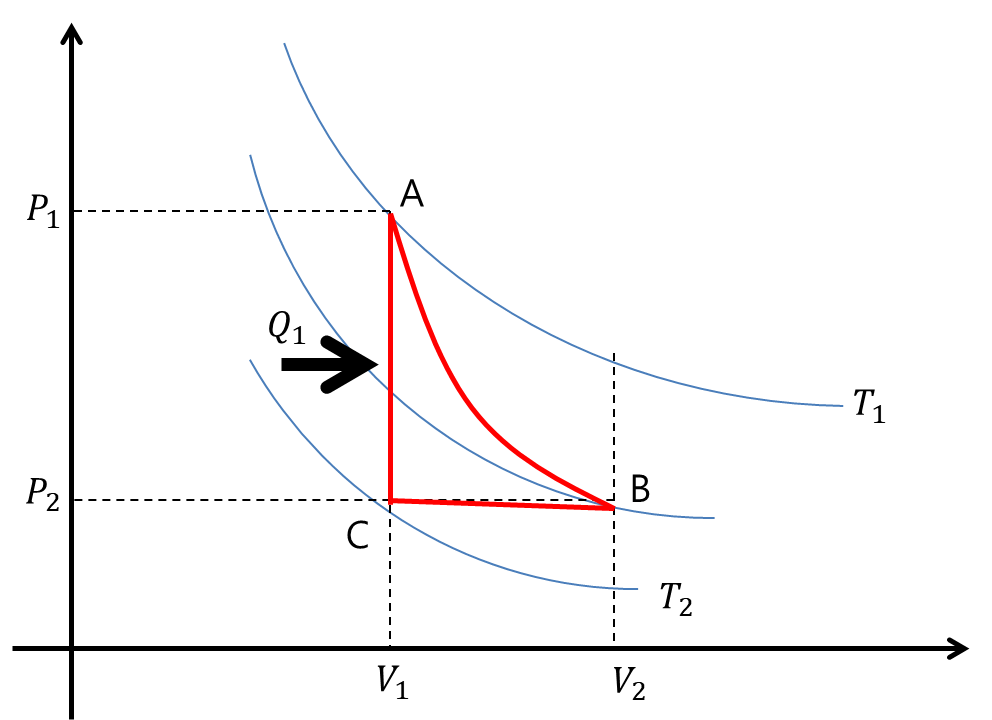
\includegraphics[width=0.5\columnwidth]{fig1.png}
		\caption{P-V 그래프}
	\end{figure}\\
	계에 준 열 $Q_1$
	$$Q_1=\frac{3}{2}P_1V_1-\frac{3}{2}P_2V_1$$
	계가 한 일
	$$\begin{cases}
	\mbox{a. 단열과정에서} (\Delta U=\Delta Q-\Delta W_1=-\Delta W_1) & \Delta W_1=-\Delta U=-\frac{3}{2}(P_2V_2-P_1V_1)\\
	\mbox{b. 등압과정에서}  & \Delta W_2=P_2(V_1-V_2)
	\end{cases}$$
	$$\Delta W=\Delta W_1+\Delta W_2=\frac{3}{2}P_1V_1-\frac{5}{2}P_2V_2+P_2V_1$$
	효율은 (한 일)/(준 열) 이므로
	$$e=\frac{\frac{3}{2}P_1V_1-\frac{3}{2}P_2V_1+\frac{5}{2}P_2V_1-\frac{5}{2}P_2V_2}{\frac{3}{2}P_1V_1-\frac{3}{2}P_2V_1}=1+\frac{5}{3}\frac{P_2V_1-P_2V_2}{P_1V_1-P_2V_1}$$
	$$=1-\frac{5}{3}\frac{(V_2/V_1-1)}{(P_1/P_2-1)}$$
	\paragraph{5-4. } 방 안 온도가 $T_L$이고 바깥 온도가 $T_H$ 일 때, 방 안으로 들어오는 열의 흡수율이 $a(T_H-T_L)$ 로 주어진다. 냉각기를 동작시켜서 같은 비율로 열을 바깥으로 내보낼 때 방 안의 온도를 구하여라. 단 냉각기의 일률은 $dW/dt$ 이다.
	\subparagraph{풀이} 냉각기의 실행계수가 
	$$K=\frac{\Delta Q}{\left|\Delta W\right|}   $$ 이므로 
	$$K=\frac{dQ/dt}{dW/dt}=\frac{T_L}{T_H-T_L}   $$n 에 열의 흡수율
	$$\frac{dQ}{dt}=a(T_H-T_L)$$ 을 대입하고 정리하면 $T_L$에 대한 2차방정식을 얻게 된다. 
	$$ a{T_L}^2-\left(2aT_H+\frac{dW}{dt} \right)T_L+a{T_H}^2=0 $$
	근의 공식을 쓰면 방 안의 온도를 다음과 같이 구할 수 있다. 
	$$T_L=T_H+\frac{1}{2a}\frac{dW}{dt}+\frac{1}{2a}\sqrt{\left( \frac{dW}{dt}\right) ^2+4aT_H\left(\frac{dW}{dt} \right) }$$
	$$\mbox{ note that, }\quad \frac{dW}{dt}<0$$
	\paragraph{5-5. } 줄-캘빈 관계식을 이용하여 절대온도 $T$를 구하고자 한다. 실험실에서는 온도에 따라 변하는 어떤 물리량 $\theta(T)$ 를 측정할 수 있으므로, 
	$$\mu'=\Maxwell[H]{\theta}{P},\quad C_P'=\Maxwell[P]{Q}{\theta},\quad \alpha'=\frac{1}{V}\Maxwell[P]{V}{\theta},\quad \frac{d\theta}{dT}$$ 등을 구할 수 있다. $T=T_0$ 일 때 $\theta(T_0)=\theta_0$  이다. 절대온도 $T$를 이들 가측정량으로 표현하여라. 
	\subparagraph{풀이}  줄-캘빈 관계식은 다음과 같이 주어진다.
	$$\mu=\Maxwell[H]{T}{P}=\frac{V}{C_P}\left[\frac{T}{V}\Maxwell[P]{V}{T}-1 \right] $$
	한편,
	$$\mu'=\Maxwell[H]{\theta}{P}=\Maxwell[H]{\theta}{T}\Maxwell[H]{T}{P}=\mu \Maxwell[H]{\theta}{T}$$
	$$C_P'=\Maxwell[P]{Q}{\theta}=\Maxwell[P]{Q}{T}\Maxwell[P]{T}{\theta}=C_P\Maxwell[P]{T}{\theta}$$
	$$\alpha'=\frac{1}{V}\Maxwell[P]{V}{\theta}=\frac{1}{V}\Maxwell[P]{V}{T}\Maxwell[P]{T}{\theta}=\alpha\Maxwell[P]{T}{\theta}$$
	의 세 관계식을 이용해서 정리하면 $\mu,\,C_P,\,\alpha$ 는 다음과 같다.
	$$\mu=\frac{\mu'}{\Maxwell[H]{\theta}{T}},\quad C_P=\frac{C_P'}{\Maxwell[P]{T}{\theta}},\quad\alpha=\frac{\alpha'}{\Maxwell[P]{T}{\theta}}$$
	주어진 줄-켈빈 관계식에 위 결과들을 넣어주면
	$$\mu=\frac{V}{C_P}\left[\frac{T}{V}\Maxwell[P]{V}{T}-1 \right] $$
	$$\frac{\mu'}{\Maxwell[H]{\theta}{T}}=\frac{V}{\frac{C_P'}{\Maxwell[P]{T}{\theta}}}\left[\frac{T\alpha'}{\Maxwell[P]{T}{\theta}}-1 \right] $$
	이므로 
	$$\mu'=\frac{V}{C_P'}\left[\alpha'T\Maxwell[P]{\theta}{T}-1 \right] $$
	에서 다음 식을 얻게 된다.
	$$\frac{1}{T}dT=\frac{\alpha'V}{V+\mu'C_P'}d\theta$$
	위 식을 적분하면
	$$\int_{T_0}^{T}\frac{1}{T'}dT'=\int_{\theta_0}^{\theta}\frac{\alpha'V}{V+\mu'C_P'}d\theta'$$
	이며, $\alpha', \mu', C_P'$ 모두 $\theta'$ 의 함수이므로 절대온도 $T$ 를 다음과 같이 얻게 된다. 
	$$ T=T_0 \,\exp\left[\int_{\theta_0}^{\theta}\frac{\alpha'V}{V+\mu'C_P'}d\theta' \right] $$
	\paragraph{5-6. } (4-7)번 문제에서 나오는 판데르 발스 기체의 몰 당 내부에너지는 $u=c_vT-a/v^2$ ($c_v$ 는 상수, $a>0$) 로 표시된다. 이 식과 상태방정식을 이용하여\\
	(ㄱ) 자유팽창 과정에서 온도가 항상 내려감을 보여라\\
	(ㄴ) 줄-톰슨 계수를 구하고 이를 이용하여 줄-톰슨 과정에서 온도가 내려갈 조건을 설명하여라.
	\subparagraph{풀이} (ㄱ) 자유팽창과정에서 $du=0$ 이므로,
	$$du=c_vdT+\frac{a}{v^2}dv=0$$
	$$c_v dT=-\frac{a}{v^2}dv,\quad \Maxwell[u]{T}{v}=-\frac{a}{v^2c_v}<0$$
	(왜냐하면 $a$와 $c_v$가 양수이기 때문에) 따라서 부피가 팽창하면 $(dv>0)$ 온도가 내려간다. $(dT<0)$\\
	(ㄴ) (5-56) 식
	$$\mu=\frac{v}{c_p}(\beta T-1)$$
	문제 (4-7)의 결과인
	$$\beta=\frac{Rv^2(v-b)}{RTv^3-2a(v-b)^2}$$
	로부터
	$$\mu=\frac{1}{c_p}\frac{2av(v-b)^2-RTv^2b}{RTv^3-2a(v-b)^2}$$ 가 된다. 이 결과를 이용하여 $\mu$의 부호를 주어진 조건으로부터 결정하면 온도가 내려갈 조건을 알 수 있다. (Reif 책 연습문제 5.20 참고) 
	\paragraph{5-7. } 용수철 상수가 $k$ 이고 길이가 $L$ 인 용수철에서 가로파동의 속도는 $\sqrt{kL/m}$ 이다. 여기서 $m$ 은 용수철의 단위길이당 질량이다. 한편 이상기체를 한쪽이 막힌 단면적이 $A$ 인 원통 속에 넣고 평형상태에서 압력과 부피를 측정하였더니 각각 $P_0,\,V_0$ 였다. 이 계를 용수철에 대응시켜서 소리의 속도를 구할 목적으로 다음과 같은 단계를 거쳤다. \\
	(ㄱ) 압력이 $P$ 이면, 이 계에 덮개가 작용하는 힘은 $PA$ 이다. 이 계에 대응하는 용수철 상수를 구하기 위하여 압력을 $dP$ 만큼 증가시켰을 때 줄어든 길이를 $dx$ 라 하자. 이 때, 계에 작용하는 힘의 증가는 $dF=\partial_V P|_0A^2dx$ 가 되어 대응하는 용수철 상수가 $k=-\partial_V P|_0A^2$ 로 주어짐을 보여라. \\
	(ㄴ) 위 결과로부터 $k=(A^2/V\chi)$ 가 됨을 보여라. 여기서 $\chi$ 는 압축률이다. \\
	(ㄷ) 소리의 속도가 $v^2=kL/m=A^2L/V\chi m=1/\chi \rho_0$ 가 됨을 보여라. 여기서 $\rho_0$ 는 이상기체의 단위 부피당 질량이다. \\
	(ㄹ) 소리의 진행 과정에서 압축은 단열과정이다. 단열압축률이 $\chi=1/\gamma P_0$ 임을 보여라. 이 결과를 이용하여 속도가 $\sqrt{\gamma P_0/\rho_0}$ 임을 보여라.
	\subparagraph{풀이} (ㄱ) $dF(x)=AdP(x)$ 이고,
	$$dP(x)=\Maxwell[0]{P}{V}dV=\Maxwell[0]{P}{V}Adx$$
	이므로,
	$$dF(x)=AdP(x)=\Maxwell[0]{P}{V}A^2dx=-kdx$$
	$$\therefore k=-\Maxwell[0]{P}{V}A^2$$
	(ㄴ)
	$$\chi=-\frac{1}{V}\Maxwell[T]{V}{P},\quad \Maxwell[T]{P}{V}=-\frac{1}{\chi V}$$
	$$k=-\Maxwell[0]{P}{V}A^2=\frac{A^2}{\chi V}$$
	(ㄷ) 
	$$v^2=\frac{kL}{m}=\frac{A^2L}{\chi V m}=\frac{1}{\chi (m/A)}$$
	$m$ 이 단위길이당 질량이므로 $(m/A)$ 는 단위부피당 질량 $\rho_0$ 로 나타낼 수 있다. 
	$$v^2=\frac{1}{\chi \rho_0}$$
	(ㄹ) 단열과정의 상태방정식
	$$PV^{\gamma}=const.$$ 에서
	$$0= V^\gamma dP+\gamma PV^{(\gamma-1)}dV$$
	$$\Maxwell[0]{V}{P}=-\left.\frac{V}{\gamma P} \right)_0=-\frac{V_0}{\gamma P_0} $$
	$$\chi=-\frac{1}{V}\Maxwell[T]{V}{P}=-\frac{1}{V_0}\left(-\frac{V_0}{\gamma P_0} \right)=\frac{1}{\gamma P_0} $$
	따라서 
	$$v=\sqrt{\frac{\gamma P_0}{\rho_0}}$$
	\paragraph{5-8. } 지구 대기권의 기체가 몰당 질량 $m$ 인 이상기체라고 가정하고, 대기에 작용하는 외부 힘은 중력뿐이고, 중력가속도 $g$ 는 일정하다고 하자.\\
	(ㄱ) 지구 표면에서 높이가 $h$ 인 곳에서 높이의 변화에 따른 압력의 변화가 $dP/P=-mgdz/(RT)$ 임을 보여라.\\
	(ㄴ) 단열 팽창으로 이러한 압력 변화가 생긴다고 가정하고, $dP/P=(\gamma/(\gamma-1))dT/T$ 이 됨을 보여라. 이 결과들로부터 $dT/dz$ 를 구해라.
	\subparagraph{풀이 } (ㄱ) 먼저 이상기체 상태방정식 $PV=nRT$ 에서 단위부피당 몰 수를 $\tilde{n}$ 라고 하면, 
	$$P=\frac{n}{V}RT=\tilde{n}RT, \quad \tilde{n}=\frac{P}{RT}$$ 
	이다. 한편 압력은 단위면적당 힘 이므로
	$$dP=dF/A$$이고, $$dF=-mg\tilde{n}dV=-mg\tilde{n}Adz$$
	따라서 $$dP=dF/A=-mg\tilde{n}dz=-mg\frac{P}{RT}dz$$
	정리하면
	$$\frac{dP}{P}=-\frac{mg}{RT}dz$$
	(ㄴ) 단열과정에서 상태방정식
	$$PT^{\gamma/(1-\gamma)}=const.$$ 을 미분하면,
	$$0=T^{\gamma/(1-\gamma)}dP+\frac{\gamma}{1-\gamma}PT^{(\gamma/(1-\gamma))-1}dT$$
	$$dP=\frac{\gamma}{\gamma-1}\frac{P}{T}dT,\quad \frac{dP}{P}=\frac{\gamma}{\gamma-1}\frac{dT}{T}$$
	(ㄱ)의 결과와 합치면
	$$\frac{dT}{dz}=-\frac{(\gamma-1)}{\gamma}\frac{mg}{R}$$
	\paragraph{5-9. } 열용량이 $C$ 로 일정한 두 열역학 계의 처음 온도가 각각 $T_1,\,T_2\,(T_1>T_2)$ 이다. 두 계를 카르노 엔진의 두 열원으로 사용했을 때 각 순환과정마다 매우 작은 일 $\dbar W$ 를 한다고 하자.\\
	(ㄱ) 이러한 카르노 엔진이 평형상태에 도달한 후, 두 계의 나중온도가 $\sqrt{T_1T_2}$ 임을 보여라. \\
	(ㄴ) 이 온도가 두 물체를 단순히 열적으로 접촉시켜서 얻게 되는 평형상태의 온도보다 높지 않음을 보여라.
	\subparagraph{풀이} (ㄱ)$$C=T\Maxwell{S}{T},\quad dS=\frac{C}{T}dT$$
	열용량이 일정한 상수라면 엔트로피 변화는 
	$$\Delta S=\int_{T_i}^{T_f}\frac{C}{T}dT=C\ln(T_f/T_i)$$ 이다. 
	카르노 엔진의 경우 두 엔진의 엔트로피 변화는 없다. 따라서 두 열원이 평형 온도 $T_e$ 에 도달했다면 각 열원의 엔트로피 변화는 
	$$\begin{cases}
	\Delta S_1=C\ln(T_e/T_1)\\\Delta S_2=C\ln(T_e/T_2)
	\end{cases}$$
	가 되는데 
	$$0=\Delta S_1+\Delta S_2 =C\ln\left(\frac{T_eT_e}{T_1T_2} \right) $$ 으로부터
	$$T_e=\sqrt{T_1T_2}$$
	(ㄴ) 단순 열접촉 시키면 $-C_1\Delta T_1=C_2\Delta T_2$ (준 열=받은 열) 에서 
	$$-C(T_e-T_1)=C(T_e-T_2),\quad T_e=\frac{T_1+T_2}{2}$$
	기하 평균이 산술 평균보다는 크지 않으므로 
	$$\frac{T_1+T_2}{2}\ge\sqrt{T_1T_2}$$
	\paragraph{5-10. } (ㄱ)
	$$TdS=C_P\Maxwell[P]{T}{V}dV+C_V\Maxwell[V]{T}{P}dP=\frac{\chi C_V}{\beta}dP+\frac{C_P}{\beta V}dV$$
	임을 보여라.\\
	(ㄴ) 이 식으로부터 단열압축률 $$\chi_S=-\frac{1}{V}\Maxwell[S]{V}{P}\,\mbox{ 이 }\quad \chi_S=\chi\frac{C_V}{C_P}=\frac{\chi}{\gamma}$$ 를 만족함을 보여라.
	\subparagraph{풀이} (ㄱ) $TdS(V,P)$ 를 변수 $V,P$ 에 대해서 전개해보자.
	\begin{equation*}
		\begin{split}
			TdS(V,P)&=T\left[\Maxwell[P]{S}{V}dV+\Maxwell[V]{S}{P}dP \right]\\
			&=T\left[\Maxwell[P]{S}{T}\Maxwell[P]{T}{V}dV+\Maxwell[V]{S}{T}\Maxwell[V]{T}{P}dP \right]\\
			&=C_P\Maxwell[P]{T}{V}dV+C_V\Maxwell[V]{T}{P}dP
		\end{split}
	\end{equation*}
	한편, 압축률과 팽창률의 정의에서,
	$$\chi=-\frac{1}{V}\Maxwell[T]{V}{P},\quad \beta=\frac{1}{V}\Maxwell[P]{V}{T}$$
	또, $\partial_PT|_V$ 를 압축률과 팽창률로 나타낼 수 있다. ($dV=0$ 인 상황)
	$$0=dV(T,P)=\Maxwell[P]{V}{T}dT+\Maxwell[T]{V}{P}dP$$
	$$\therefore0=\beta VdT-\chi VdP,\quad \Maxwell[V]{T}{P}=\frac{\chi}{\beta}$$
	따라서,
	$$TdS(V,P)=C_P\Maxwell[P]{T}{V}dV+C_V\Maxwell[V]{T}{P}dP$$
	$$=\frac{C_P}{\beta V}dV+\frac{\chi C_V}{\beta}dP$$
	(ㄴ) $\dbar Q=TdS=0$ 인 단열과정에서는 (ㄱ) 의 결과로부터
	$$0=\frac{C_P}{\beta V}dV+\frac{\chi C_V}{\beta}dP $$
	에서
	$$\chi_S=-\frac{1}{V}\Maxwell[S]{V}{P}=\frac{\frac{\chi C_V}{V\beta}}{\frac{C_P}{\beta V}}=\chi\frac{C_V}{C_P}=\frac{\chi}{\gamma}$$
	\chapter*{6장 작은 바른틀 앙상블}
	\paragraph{6-1. } $N$ 개의 상태 중 $i$ 상태에 있을 확률이 $p_i$ 이고 규격화조건 $\sum_{i=1}^{N}p_i=1$ 을 만족한다. 라그랑주의 미정계수법을 이용하여 최대 엔트로피가 $S_m=k_B\ln N$ 임을 보여라.
	\subparagraph{풀이} 엔트로피의 정의식 
	$$S=-k_B\sum_{i=1}^{N}p_i\ln{p_i}$$
	을 주어진 constraint인 $\sum_{i=1}^{N}p_i=1$ 의 조건에 따라 최대값을 구해야 한다.\\
	라그랑주의 미정계수를 $\lambda$ 라고 하자.
	$$\begin{cases}
	dS=-k_B\sum_{i=1}^{N}(\ln{p_i}+1)dp_i\\
	0=\lambda\sum_{i=1}^{N}dp_i
	\end{cases}$$
	교과서에서 한 것처럼 둘을 더하면,
	$$dS=-k_B\sum_{i=1}^{N}(\ln p_i+1-\lambda)dp_i$$
	최대의 조건에서 $dS=0$ 이므로 $\ln p_i=\lambda-1$ 을 만족해야 한다. 또는
	$$p_i=e^{\lambda-1}=const.$$
	을 만족해야 한다. 바꿔말하면, 모든 $p_i$ 는 서로 같으며 규격화조건을 고려하면 모든 확률은 
	$$p_i=\frac{1}{N}$$
	이 된다. 따라서 최대 엔트로피는 
	$$S=-k_B\sum_{i=1}^{N}p_i\ln{p_i}=-k_BN\left(\frac{1}{N}\ln\frac{1}{N}\right)=k_B\ln N$$
	\paragraph{6-2. } 이상기체의 Sackur-Tetrode 방정식을 이용하여 서로 구별할 수 있는 두 이상기체를 섞거나 서로 구별할 수 없는 이상기체를 섞거나 상관없이 깁스의 역리가 생기지 않음을 보여라. 
	\subparagraph{풀이} 서로 구별할 수 있는 입자의 Sackur-Tetrode 방정식\\  단, 단위 입자당 에너지는 $u=(3/2)k_BT$  이다. 
	$$S(E,V,N)\simeq Nk_B\left[\frac{3}{2}+\ln\left[V\left(\frac{4\pi mE}{3Nh^2} \right)^{3/2}  \right]  \right]=Nk_B\left[\frac{3}{2}+\ln\left[V\left(\frac{4\pi mu}{3h^2} \right)^{3/2}  \right]  \right] $$
	서로 구별할 수 없는 입자의 Sackur-Tetrode 방정식
	$$S(E,V,N)\simeq Nk_B\left[\frac{5}{2}+\ln\left[\frac{V}{N}\left(\frac{4\pi mE}{3Nh^2} \right)^{3/2}  \right]  \right]=Nk_B\left[\frac{5}{2}+\ln\left[\frac{V}{N}\left(\frac{4\pi mu}{3h^2} \right)^{3/2}  \right]  \right] $$
	(\romannumeral 1) 두 입자를 서로 구별할 수 있는 경우에 처음상태와 나중상태의 엔트로피는 다음과 같다. 
	$$S_i=S_1(T,V_1,N_1)+S_2(T,V_2,N_2),\quad S_f=S_1(T,V_1+V_2,N_1)+S_2(T,V_1+V_2,N_2)$$
	\begin{equation*}
		\begin{split}
		S_i&=S_1(T,V_1,N_1)+S_2(T,V_2,N_2)\\
		&=N_1k_B\left[\frac{3}{2}+\ln\left[V_1\left(\frac{4\pi mu}{3h^2} \right)^{3/2}  \right]  \right]+N_2k_B\left[\frac{3}{2}+\ln\left[V_2\left(\frac{4\pi mu}{3h^2} \right)^{3/2}  \right]  \right]\\
		S_f&=S_1(T,V_1+V_2,N_1)+S_2(T,V_1+V_2,N_2)\\
		&=N_1k_B\left[\frac{3}{2}+\ln\left[(V_1+V_2)\left(\frac{4\pi mu}{3h^2} \right)^{3/2}  \right]  \right]+N_2k_B\left[\frac{3}{2}+\ln\left[(V_1+V_2)\left(\frac{4\pi mu}{3h^2} \right)^{3/2}  \right]  \right]
		\end{split}
	\end{equation*}
	따라서 엔트로피 변화는 
	\begin{equation*}
		\begin{split}
		\Delta S&=S_f-S_i\\
		&=N_1k_B\ln\left(\frac{V_1+V_2}{V_1} \right)+N_2k_B\ln\left( \frac{V_1+V_2}{V_2}\right) >0 
		\end{split}
	\end{equation*}
	엔트로피의 변화가 양수로, 입자들을 구별할 수 있을 때 두 기체를 섞는 행동은 비가역과정이다. (교과서 80쪽)\\
	(\romannumeral 2) 두 입자를 서로 구별할 수 없는 경우에 처음상태와 나중상태의 엔트로피는 다음과 같다. 
	$$S_i=S_1(T,V_1,N_1)+S_2(T,V_2,N_2),\quad S_f=S(T,V_1+V_2,N_1+N_2)$$
	\begin{equation*}
		\begin{split}
		S_i&=S_1(T,V_1,N_1)+S_2(T,V_2,N_2)\\
		&=N_1k_B\left[\frac{5}{2}+\ln\left[\frac{V_1}{N_1}\left(\frac{4\pi mu}{3h^2} \right)^{3/2}  \right]  \right]+N_2k_B\left[\frac{5}{2}+\ln\left[\frac{V_2}{N_2}\left(\frac{4\pi mu}{3h^2} \right)^{3/2}  \right]  \right]
		\end{split}
	\end{equation*}
	\begin{equation*}
	\begin{split}
	S_f&=S(T,V_1+V_2,N_1+N_2)\\
	&=(N_1+N_2)k_B\left[\frac{5}{2}+\ln\left[\frac{V_1+V_2}{N_1+N_2}\left(\frac{4\pi mu}{3h^2} \right)^{3/2}  \right]  \right]
	\end{split}
	\end{equation*}
		따라서 엔트로피 변화는 
	\begin{equation*}
	\begin{split}
	\Delta S&=S_f-S_i\\
	&=(N_1+N_2)k_B\ln\frac{V_1+V_2}{N_1+N_2}-N_1k_B\ln\frac{V_1}{N_1}-N_2k_B\ln\frac{V_2}{N_2}
	\end{split}
	\end{equation*}
	인데, 동등입자의 밀도는 항상 같으므로
	$$\frac{V_1}{N_1}=\frac{V_2}{N_2}=\frac{V_1+V_2}{N_1+N_2}$$
	결국 $\Delta S=0$ 인 가역과정이다. 동등입자의 경우 위와 같이 두 기체를 섞는 행동은 가역과정이다. 깁스의 역리 (Gibbs Paradox)란 동등입자 계를 계산했을 때 엔트로피 변화가 양수가 되어 가역과정임에도 비가역과정으로 나타나는 현상이다. Sackur-Tetrode 방정식은 깁스의 역리가 생기지 않으므로 이상기체를 서술하는 올바른 방정식임을 알 수 있다.  
	\paragraph{6-3. } Sackur-Tetrode 방정식을 이용해서 열역학 함수 $E,\,F,\,H,\,G$ 를 구하여라.
	\subparagraph{풀이} (ㄱ) Sackur-Tetrode 방정식
	$$S(U,V,N)\simeq Nk_B\left[\frac{5}{2}+\ln\left[\frac{V}{N}\left(\frac{4\pi mU}{3Nh^2} \right)^{3/2}  \right]  \right]$$
	을 정리하여 내부에너지로 표기하면 다음과 같다.
	$$U(S,V,N)=\frac{3Nh^2}{4\pi m}\left(\frac{N}{V} \right)^{2/3}\exp\left[\frac{2S}{3Nk_B}-\frac{5}{3} \right]  $$
	한편,
	$$T=\Maxwell[N,V]{U}{S}=\frac{2}{3Nk_B}U$$ 에서 $U=(3/2)k_BT$ 를 확인할 수 있다. \\
	(ㄴ) 자유에너지는 $F=U-TS$ 이므로 다음과 같다.
	\begin{equation*}
		\begin{split}
		F&=U-Nk_BT\left[\frac{5}{2}+\ln\left[\frac{V}{N}\left(\frac{4\pi mU}{3Nh^2} \right)^{3/2}  \right]   \right] \\
		&=Nk_BT\left[-1-\ln\left[\frac{V}{N}\left(\frac{2\pi m k_B T}{h^2} \right)^{3/2} \right]  \right] 
		\end{split}
	\end{equation*}
	로그 안의 분모 분자를 바꾸면,
	$$=Nk_BT\left[\ln\left[\frac{N}{V}\left(\frac{h^2}{2\pi m k_B T} \right)^{3/2} \right]  -1\right]$$
	let $n=\frac{N}{V}, \quad \lambda=\left(\frac{h^2}{2\pi m k_B T} \right)^{1/2} $ 
	$$=Nk_BT\left[\ln(n \lambda ^{3} )  -1\right]$$
	$$F=Nk_BT\left[\ln(n \lambda ^{3} )  -1\right]$$
	(ㄷ) $H=U+PV$ 이므로 먼저 $P$ 를 구하면
	$$-P=\Maxwell[S,N]{U}{V}=-\frac{2}{3V}U$$
	이므로 엔탈피는 다음과 같다. 
	$$H=U+PV=\frac{5}{3}U=\frac{5Nh^2}{4\pi m}\left(\frac{N}{V} \right)^{2/3}\exp\left[\frac{2S}{3Nk_B}-\frac{5}{3} \right]  $$
	(ㄹ) Gibbs free energy는 $G=U-TS+PV=F+PV$ 에서
	$$G=Nk_BT[\ln(n\lambda^3)-1]+PV=Nk_BT\ln(n\lambda^3)$$
	\paragraph{6-4. } 어떤 계의 확률분포가 
	$$p(x)=\frac{1}{\sqrt{2\pi \sigma^2}}\,e^{-\frac{x^2}{2\sigma^2}},\quad -\infty\le x \ge \infty$$
	로 주어질 때, 계의 엔트로피를 구하여라. 
	\subparagraph{풀이} 엔트로피의 정의식 $S=-k_B\sum p_i \ln p_i$ 에서 다음과 같이 구할 수 있다. 
	\begin{equation*}
		\begin{split}
		S&=-k_B\int_{-\infty}^{\infty}p(x)\ln p(x) dx\\
		&=-k_B\int_{-\infty}^{\infty}p(x)\left(-\ln\sqrt{2\pi\sigma^2}-\frac{x^2}{2\sigma^2} \right) dx\\
		&=k_B\ln\sqrt{2\pi \sigma^2}\int_{-\infty}^{\infty}p(x)dx+\frac{k_B}{2\sigma^2}\int_{-\infty}^{\infty}x^2p(x)dx
		\end{split}
	\end{equation*}
	한편 규격과조건과 2차 모먼트는 다음과 같다.
	$$\int_{-\infty}^{\infty}p(x)dx=1$$
	$$\int_{-\infty}^{\infty}x^2p(x)dx=\frac{1}{\sqrt{2\pi\sigma^2}}\int_{-\infty}^{\infty}x^2\exp\left(-\frac{x^2}{2\sigma^2} \right)dx=\sigma^2 $$
	따라서
	$$S=k_B\ln\sqrt{2\pi\sigma^2}+\frac{k_B}{2}$$
	\paragraph{6-5. } 두 개의 양자 준위 $-\epsilon,\epsilon$ 을 갖는 $N$ 개의 상호작용하지 않는 입자로 구성된 고립계가 있다. 이 계의 내부에너지가 $U=M\epsilon$ $(M=-N,\cdots,N)$ 일 때 계의 엔트로피를 구하고 그것으로부터 계의 온도를 구하여라. 이 계가 $M>0$ 일 때 생기는 모순을 발견하고 물리적인 해결 방법을 설명해라.
	\subparagraph{풀이} 준위 $\epsilon$ 에 있는 입자의 갯수를 $n_1$, 준위 $-\epsilon$ 에 있는 입자의 갯수를 $n_2$ 라고 하면
	$$\begin{cases}
	n_1+n_2=N\\
	n_1-n_2=M
	\end{cases}$$
	이므로
	$$\begin{cases}
	n_1=(N+M)/2\\n_2=(N-M)/2
	\end{cases}$$
	따라서 계의 상태수 $\Omega$ 는 
	$$\Omega=\frac{N!}{[(N+M)/2]![(N-M)/2]!}$$
	이다. 엔트로피는 $S=Nk_B\ln \Omega$ 에서
	\begin{equation*}
		\begin{split}
			S&=k_B[\ln N!-\ln[(N+M)/2]!-\ln[(N-M)/2]!]\\
			&=k_B\left[N\ln N-N-\left(\frac{N+M}{2}\ln\frac{N+M}{2}+\frac{N-M}{2}\ln\frac{N-M}{2}-N \right) \right]\\
			&=k_B\left[N\ln N-\frac{N+M}{2}\ln\frac{N+M}{2}+\frac{N-M}{2}\ln\frac{N-M}{2}\right]
		\end{split}
	\end{equation*}
	가 된다. 온도의 정의
	$$\frac{1}{T}=\Maxwell[]{S}{U}=\Maxwell{S}{M}\Maxwell{M}{U}=\frac{1}{\epsilon}\Maxwell{S}{M}$$으로부터
	$$\frac{1}{T}=\frac{k_B}{2\epsilon}\ln\left(\frac{N-M}{N+M} \right)=\frac{k_B}{2\epsilon}\ln\left(1-\frac{2M}{N+M} \right)  $$ 
	$M$ 이 $0$ 보다 큰 경우에는 절대온도가 음수가 되는 모순이 생기는데, 이러한 경우가 고립된 상자성 이징 모형이다. 따라서 이러한 계는 독립적으로 존재하지 않고 다른 열역학계와 결합되어 있어서 항상 절대온도가 $T>0$ 을 만족시켜주어야 한다. 
	\paragraph{6-6. } 넓이가 $A$ 인 2차원의 네모꼴 내부에 국한된 이상기체가 있다. 작은 바른틀 앙상블을 이용하여 이상기체의 상태방정식 및 내부에너지를 구하여라. 
	\subparagraph{풀이} Note that the volume of $N$-dimensional sphere with radius $R$ is
	$$V=C_NR^N=\frac{\pi^{N/2}}{\frac{N}{2}\left(\frac{N}{2}-1 \right)! }R^N$$
	이 경우 계의 $\Sigma(E)$ 는
	$$\Sigma(E)=\frac{1}{N!h^{2N}}\int_{H\le E}d^{2N}qd^{2N}p=\frac{A^N}{N!h^{2N}}\int_{H\le E}d^{2N}p$$
	위의 $N$ 차원 구의 부피 공식을 쓰면,
	$$\Sigma(E)=\frac{A^N}{N!h^{2N}}\frac{\pi^N}{N(N-1)!}(2mE)^N$$
	$\Sigma$ 를 미분하면
	$$\Omega(E)=\frac{\partial \Sigma}{\partial E}dE=\frac{A^N}{N!h^{2N}}\frac{(2m\pi)^N}{(N-1)!}E^{N-1}dE$$
	$$\simeq\frac{A^N}{N!N!h^{2N}}(2m\pi E)^N$$
	따라서 계의 엔트로피는 
	\begin{equation*}
		\begin{split}
		S=k_B\ln{\Omega}&=k_B\left(\ln\left[\frac{2m\pi AE}{h^2} \right]^N-2(\ln N!)  \right)\\
		&=k_B\left(\ln\left[\frac{2m\pi AE}{h^2} \right]^N-2(N\ln N-N) \right)  \\
		&=Nk_B\left(\ln \left[\frac{2m\pi AE}{N^2h^2} \right]+2  \right) 
		\end{split}
	\end{equation*}
	따라서 상태방정식과 내부에너지는 각각
	$$\Maxwell[U]{S}{A}=\frac{P}{T}=\frac{Nk_B}{A}\rightarrow PA=Nk_BT $$
	$$\Maxwell[A]{S}{U}=\frac{1}{T}=\frac{Nk_B}{E}\rightarrow E=Nk_BT$$
	\paragraph{6-7. } 1차원 살창구조에서 $N$ 개의 살창자리에 어떤 분자가 흡착될 때의 에너지는 $\epsilon\,(\epsilon>0)$ 이다. $\bar{N}\,(\bar{N}<N)$ 개의 분자가 흡착되어 있을 때, 작은 바른틀 앙상블을 이용하여 내부에너지와 온도와의 관계를 구하여라.
	\subparagraph{풀이} 이 계의 에너지는 $U=-\bar{N} \epsilon$ 이고 number of accesible states $\Omega$ 는
	$$\Omega=\frac{N!}{\bar{N}!(N-\bar{N})!}$$
	에서 엔트로피는 
	$$S=k_B\ln\Omega=k_B[(N\ln N-N)-(\bar{N}\ln\bar{N}-\bar{N}+(N-\bar{N})\ln(N-\bar{N})-N+\bar{N})]$$
	$$=k_B[N\ln N-\bar{N}\ln\bar{N}-(N-\bar{N})\ln(N-\bar{N})]$$
	온도의 정의에서
	$$\frac{1}{T}=\frac{\partial S}{\partial U}=\frac{\partial S}{\partial \bar{N}}\frac{\partial \bar{N}}{\partial U}=-\frac{1}{\epsilon}\frac{\partial S}{\partial \bar{N}}$$
	$$=-\frac{1}{\epsilon}k_B(-\ln \bar{N}-1+\ln(N-\bar{N})+1)$$
	$$=-\frac{k_B}{\epsilon}\left(\ln\frac{N-\bar{N}}{\bar{N}} \right)=\frac{k_B}{\epsilon}\left(\ln\frac{\bar{N}}{N-\bar{N}} \right)  $$
	로그의 양변에 $\epsilon$ 을 곱하면
	$$\frac{1}{T}=\frac{k_B}{\epsilon}\left(\ln\frac{\epsilon\bar{N}}{\epsilon N-\epsilon\bar{N}} \right)=\frac{k_B}{\epsilon}\left(\ln\frac{-U}{\epsilon N+U} \right) $$
	\paragraph{6-8. } $N$ 개의 주사위를 던져서 나올 수 있는 방법의 수를 생각할 때, 주사위가 균일한 재질로 구성되어 있다면, $N\rightarrow\infty$ 인 극한에서는 1부터 6까지 나올 확률은 모두 같은 것이 가장 자연스럽다는 것을 보여라.
	\subparagraph{풀이} 만약 각 주사위의 모든 눈이 나올 확률이 동일하다면 가능한 방법의 수는 $\Omega=6^N$ 이다. 그런데 어느 주사위 하나라도 가능한 6가지 눈 중 한 눈이라도 나올 확률이 사라지면 그 때의 $\Omega$ 는 $5\times6^{(N-1)}$ 로 줄어든다. 이는 $N\rightarrow\infty$ 에서는 엔트로피라는 측면에서 볼 때 불가능하므로 1부터 6까지 나올 확률은 모두 같은 것이 가장 자연스럽다는 것이 증명된다. 이러한 법칙을 최대 불확실 법칙(Maximum Uncertainty Principle) 이라 부른다. 이러한 논법의 수학적 증명이 바로 (6-1) 번 문제라 할 수 있다. 
	
	\chapter*{7장 바른틀 앙상블}
	\paragraph{7.1 } $N$ 개의 상태 중 $i$ 상태에 있을 확률이 $p_i$ 이고 규격화조건 $\sum_{i=1}^{N}p_i=1$ 을 만족한다. $i$ 상태에서 거시변수 $x$ 가 $x_i$ 이고 그 평균값이 $x_0=\sum_{i=1}^{N}p_ix_i$ 일 때, 라그랑주의 미정계수법을 이용하여 최대 엔트로피가 $S_m=k_B\beta x_0+k_B\ln Z$ 임을 보여라. 단 $\beta$ 는 미정계수 중 하나이고, $Z(x)=\sum_{i} e^{-\beta x_i}$
	\subparagraph{풀이} 엔트로피의 정의식 
	$$S=-k_B\sum_{i=1}^{N}p_i\ln p_i$$ 를 주어진 constraint
	$$\sum_{i=1}^{N}p_i=1,\quad\sum_{i=1}^{N}p_ix_i=x_0$$
	에 따라서 최대값을 구해야 한다. 따라서 두 개의 라그랑주 미정계수를 $\alpha,\,\beta$ 라고 놓으면
	$$\begin{cases}
	dS=-k_B\sum_{i}(\ln p_i+1)dp_i\\
	0=\sum_{i}\alpha dp_i\\
	0=\sum_{i}-\beta x_i dp_i
	\end{cases}$$
	밑의 두 식에 $k_B$ 씩 곱하고 더하면,
	$$dS=-k_B\sum_{i=1}^{N}(\ln p_i+1-\alpha+\beta x_i)$$
	이 $dS$ 가 0이 될 때 최댓값을 가지므로 
	$$\ln p_i+1-\alpha+\beta x_i=0$$
	에서
	$$p_i=e^{\alpha-1}e^{-\beta x_i}$$ 이 되고, 규격화조건 $\sum_i p_i=1$ 에서 다음과 같다. 
	$$1=\sum_{i=1}^{N}p_i=e^{\alpha-1}\sum_{i=1}^{N}e^{-\beta x_i}=e^{\alpha-1}Z(x),\quad Z(x)=\sum_{i=1}^{N}e^{-\beta x_i}$$
	$$\therefore e^{\alpha-1}=\frac{1}{Z},\quad p_i=\frac{e^{-\beta x_i}}{Z}$$
	따라서 최대 엔트로피는 다음과 같다. 
	\begin{equation*}
		\begin{split}
		S=-k_B\sum_{i=1}^{N}p_i\ln p_i&=-k_B\sum_{i=1}^{N}p_i\ln\left(\frac{e^{-\beta x_i}}{Z} \right) \\
		&=k_B\sum_{i=1}^{N}\beta p_ix_i+k_B\sum_{i=1}^{N}p_i\ln Z\\
		&=k_B\beta x_0+k_B\ln Z
		\end{split}
	\end{equation*}
	\paragraph{7.2 } 에너지 값이 $E_n=(n+1/2)\hbar \omega$ 로 주어지는 1차원 조화진동자가 온도 $T$ 인 열원과 열적으로 접촉하고 있다.\\
	(ㄱ) 평균 에너지 $\langle E\rangle$ 를 구하여라\\
	(ㄴ) $\langle (\Delta E)^2 \rangle$ 를 구하여라
	\subparagraph{풀이} Note that
	$$\langle E\rangle=-\frac{\partial \ln Z}{\partial \beta},\quad \langle (\Delta E)^2 \rangle=\frac{\partial^2(\ln Z)}{\partial \beta^2}$$
	먼저 분배함수 $Z$ 를 구하자.
	\begin{equation*}
		\begin{split}
			Z=\sum_{n}e^{-\beta E_n}&=\sum_{n}e^{-(n+1/2)\beta\hbar\omega}\\
			&=e^{-\frac{1}{2}\beta\hbar\omega}\sum_{n}e^{-n\beta\hbar\omega}\\
			&=e^{-\frac{1}{2}\beta\hbar\omega}\left(\frac{1}{1-e^{-\beta\hbar\omega}} \right) 
		\end{split}
	\end{equation*}
	 또는
	$$\ln Z=-\frac{1}{2}\beta\hbar\omega-\ln(1-e^{-\beta\hbar\omega})$$
	\paragraph{7.3 }
	\subparagraph{풀이}
	\paragraph{7.4 }
	\subparagraph{풀이}
	\paragraph{7.5 }
	\subparagraph{풀이}
	\paragraph{7.6 }
	\subparagraph{풀이}
	\paragraph{7.7 }
	\subparagraph{풀이}
	\paragraph{7.8 }
	\subparagraph{풀이}
	\paragraph{7.9 }
	\subparagraph{풀이}
	\paragraph{7.10 }
	\subparagraph{풀이}
	\paragraph{7.11 }
	\subparagraph{풀이}
\end{document}